\documentclass[../CMPUT-404-Notes.tex]{subfiles}
\begin{document}
\chapter{AJAX}

\begin{DndSidebar}[color=PhbLightGreen]{What is AJAX}
    \textbf{AJAX} stands for \textbf{Asynchronous JavaScript and XML}, although XML has been replaced by JSON.

    \begin{itemize}
        \item Client Side
        \item Allows Javascript to make HTTP requests and use the results without redirecting the browser.
        \item Enables heavy-clients and lightweight webservices
        \item Can be used to avoid presentation responsibility on the webservice.
        \item JSON is a common replacement for XML
        \item Twitter.com is heavy on Ajax
    \end{itemize}
\end{DndSidebar}

AJAX is great an all but has its issues.
\begin{itemize}
    \item You have to manage History, Back button, Bookmarks in JS
    \item Security: browsers heavily restrict AJAX to prevent abuse, has Same-Origin Policy
    \item Even more HTTP requests, consuming more CPU and RAM resources.
\end{itemize}

\section{Making Requests}
Use JS to make a HTTP request and get the content
The old school way of doing that was to use:
\begin{minted}[breaklines]{javascript}
new XMLHttpRequest()
\end{minted}
The new way is to use the \texttt{Fetch} API
\begin{minted}[breaklines]{javascript}
promise = new Request("some-url");
\end{minted}

When you use the \texttt{Fetch} API it returns a \texttt{Promise} object which represents the eventual completion (or failure) of an asynchronous operation and its resulting value.

\subsection{Promise}
When you make a \mintinline{javascript}{new Request()} it returns a Request object, that Request object can be asynchronously executed by calling \mintinline{javascript}{fetch(request)} on the request. This will create a "pending" Promise object. Once created that request will be put into a queue waiting to be asynchronous processed. Once processed or rejected it will then run a callback function given as a argument of the \texttt{then()} method of the promise object. 

\texttt{then()} can take in two callback functions, the first function being called on a successful operation, and the second function being called on a failed operation. 
Both callback functions can be optional, and are replaced with an identity function if not specified. 
The returning object from a \texttt{then()} method is another promise. This allows users to chain promises together. 


\subsubsection{Example}
\begin{minted}[breaklines]{javascript}
function makeAPromise(data) {
  return new Promise((resolve, reject) => {
    resolve(data);
  });
}
function promiseExample() {
  // .then returns a NEW promise
  var promise1 = makeAPromise("X");
  var promise2 = promise1.then((data2) => {
    // inner function gets called after the promise is resolved
    alert("data2: " + data2);
    return "Y";
  });
  // .then calls its argument with the return value of the
  //     previous promises's callback function
  var promise3 = promise2.then((data3) => {
    alert("data3: " + data3);
  });
}
\end{minted}
In the \mintinline{javascript}{promiseExample()} the first promise is to resolve the value "X", then makes another promise to alert the user that data2 is X, where it will return the value "Y". After which is another promise to promise3 where it will alert the user with data3 is Y.

\section{Promise dot-chaining}
You can also dot-chain or cascade promises into one another. 
\begin{minted}[breaklines]{javascript}
  var request = new Request("images/fetch.gif");
  var promise1 = fetch(request);
  var promise2 = promise1.then(function(response) {
    console.log("Got headers!");
    return response.blob(); // return a promise for raw binary data
  });
  promise2.then(function(blob) {
    console.log("Got data blob!");
    var objectURL = URL.createObjectURL(blob);
    img.src = objectURL;
  });
}
\end{minted}

is the same as 

\begin{minted}[breaklines]{javascript}
var request = new Request("images/fetch.gif");
fetch(request).then(function(response) {
  console.log("Got headers!");
  return response.blob(); // return a promise for raw binary data
}).then(function(blob) {
  console.log("Got data blob!");
  var objectURL = URL.createObjectURL(blob);
  img.src = objectURL;
});
\end{minted}


\section{Fetching JSON}
This is a generic JSON GET function
\begin{minted}[breaklines]{javascript}
function fetchJSON(url) {
  var request = new Request(url);
  return fetch(request).then((response) => {
    if (response.status === 200) { // OK
      return response.json(); // return a Promise
    } else {
      alert("Something went wrong: " + response.status);
    }
  });
}

var getterID; // global
// Get some JSON every second
function startGetting() {
  getterID = window.setInterval(() => { // callback
    var now = new Date();
    var s = 1 + (now.getSeconds() % 4); // remainder
    var url = s + ".json" // 1.json 2.json 3.json...
    fetchJSON(url).then((json) => { // another callback
      console.log(json); // browser turned the JSON into an object
      text = json.message; // it has properties
      document.querySelector("#ajaxy").innerText = text;
    });
  }, 1000); // 1 second or 1000ms
}
function stopGetting() {
  window.clearInterval(getterID);
}
\end{minted}

This code will fetch a JSON object as a promise and return the content of the JSON as another promise to be process/read. The third promise is not consumed or used. 
The content of the JSON file is put into blockquotes using DOM manipulation.
A new content is put into the blockquotes after a second or so.

\begin{minted}[breaklines]{html}
<button type="button" onclick="startGetting()">Start Getting</button>
<button type="button" onclick="stopGetting()">Stop Getting</button>
<blockquote id="ajaxy"></blockquote>
\end{minted}

\subsection{Timers}

\begin{itemize}
    \item \mintinline{javascript}{window.setInterval} lets you run a function every so many milliseconds.
    \item \mintinline{javascript}{window.setTimeout} lets you run a function once after so many milliseconds.
\end{itemize}

\begin{Note}
    These timers are not accurate and are not designed to be accurate.
\end{Note}

\section{JSON}
\begin{DndSidebar}[color=PhbLightGreen]{JSON}
    \begin{itemize}
        \item JavaScript Object Notation
        \item Strict subset of JavaScript
        \item \texttt{JSON.parse} parses JSON text into an Object
        \item \texttt{JSON.stringify} turns an Object into JSON text
    \end{itemize} 

\end{DndSidebar}

\subsubsection{Example}
\begin{minted}[breaklines]{javascript}
function stringifyExample() {
  var obj = { "food":"hotdog", 
              "condiments":["ketchup","mustard","cheese"],
              "sausage":"weiner"
  };
  document.querySelector("#hotdog").value = 
    JSON.stringify(obj, null, " "); // pretty print
}
function parseExample() {
  text = document.querySelector("#hotdog").value;
  var newObj = JSON.parse(text); 
  document.querySelector("#sausage").innerText = newObj.sausage;
}
\end{minted}

\section{Design with AJAX}
The design goal of AJAX is to minimize AJAX requests and traffic by bundling together request, etc.
Don't hook into every event, use timeouts. 
This was use to ease page state transition.
\\~\\
What are your events?
\begin{itemize}
    \item Per user input?
    \item Per user commit?
    \item Time based?
    \item Per Server action?
    \item Polling?
    \item Data?
    \item Content oriented?
    \item Messages?
    \item Multimedia?
    \item Read-based (reddit)
\end{itemize}

\section{AJAX Observer Pattern}
\begin{DndSidebar}[color=PhbLightGreen]{Observer Pattern}
    Observer pattern is where an observable keeps a collection of observers (listeners) and notifies those observers if anything changed by sending an update message.
\end{DndSidebar}
This works great with AJAX if the observable is held client side in a browser and the observer is client side in the browser! Go ahead!

\begin{figure}[htbp]
    \centering
    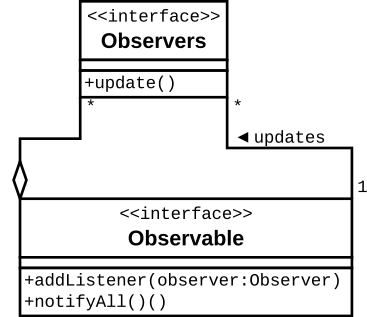
\includegraphics[width=0.8\columnwidth]{../assets/observer.png}
    \caption{Observer Pattern UML}
    \label{fig:observer-pat}
\end{figure}

\begin{itemize}
    \item Still works well with observable in browser and the observers server-side, the client simply notifies via the server's observers whenever an update occurs (but it should also communicate some lightweight state).
    \item  Due to the lack of a client-side HTTP server it is problematic to do the observer pattern with client side observers.
\end{itemize}

\subsection{Observing the Server}
HTTP is stateless, so a client needs to communicate somehow all of the objects it is observing.
Perhaps a serverside Observer proxy that stores observables for a client.
Clients need to poll the server to check if there are updates. For the observer pattern to work this polling should allow the server to send update commands.
Due to bandwidth concerns and latency concerns, an update from the server should probably include relevant data.
\\~\\
Fighting against:
\begin{itemize}
    \item Latency
    \item Bandwidth
    \item Lack of communication channels 
    \item Lack of ability to push messages to a client 
    \item Polling
    \item Timer smashing
\end{itemize}
Solution?
\begin{itemize}
    \item Polling: The most common 
    \item Push API: Not supported on all browsers 
    \item Comet "long polling": Difficult server-side support 
    \item Websockets: need to make a websocket server.
\end{itemize}

\subsection{Polling the Server}
\begin{itemize}
    \item Don't send too many requests
    \item Batch (bundle together) requests to the server
    \item Minimize the number of timers and the frequency of timers
    \quad E.g. if drawing, a user doesn't need more than 30FPS!
    \item Don't make requests until the previous request finished...
    \item Don't make requests you don't have to
\end{itemize}


\section{Async and Await}
The \mintinline{javascript}{async} and \mintinline{javascript}{await} are JavaScript keywords that makes asynchronous code easier to write and read afterwards.

\begin{itemize}
  \item \mintinline{javascript}{async} functions returns a promise
  \item \mintinline{javascript}{await} in the async function blocks code execution (stop and wait for the promise to resolve).
\end{itemize}

\subsubsection{Example}
\begin{minted}[breaklines]{javascript}
var getterID; // global
async function get2() {
  var now = new Date();
  var s = 1 + (now.getSeconds() % 4); // remainder
  var url = s + ".json" // 1.json 2.json 3.json...
  var json = await fetchJSON(url);
  console.log(json); // browser turned the JSON into an object
  var text = json.message; // it has properties
  document.querySelector("#ajaxy2").innerText = text;
}
function startGetting2() {
  getterID2 = window.setInterval(get2, 1000); // 1 second or 1000ms
}
function stopGetting2() {
  window.clearInterval(getterID2);
}
\end{minted}

\begin{minted}[breaklines]{html}
<button type="button" onclick="startGetting2()">Start Getting</button>
<button type="button" onclick="stopGetting2()">Stop Getting</button>
<blockquote id="ajaxy2"></blockquote>
\end{minted}

\subsection{Disadvantages}
\begin{itemize}
  \item Execution stops at await, instead of continuing in parallel, although if the browser supports threads then the waiting execution will be threaded.
  \item with \mintinline{javascript}{.then(...)} in a loop, the loop completes instantly and each callback function can run in parallel as soon as its ready
  \item With \mintinline{javascript}{await} in a loop, the loop will keep stopping each time in gets to the await. 
\end{itemize}


\section{Review}
\paragraph{AJAX}
\begin{itemize}
  \item Asynchronous JavaScript and XML now JSON
  \item Allows JS to make HTTP request and use the result without redirecting
  \item A lot of websites uses AJAX
  \item The goal of using AJAX is to minimize AJAX requests and traffic by either bundling requests together, etc
\end{itemize}
\paragraph{XMLHttpRequest}
\begin{itemize}
  \item The the old school of making async requests. 
  \item You have to setup an \mintinline{javascript}{onreadystatechange()} function as an event handler and
  \item have to process a lot of things by yourself  
\end{itemize}
\paragraph{Request}
\begin{itemize}
  \item Is the new, modern way of doing things. 
  \item It will handle all the state changes and event handlers and all you need to do is implement the promise's handler or callback function. 
  \item \mintinline{javascript}{new Request("url")} will create a request object that is the interface for the Fetch API. 
  \item Calling \mintinline{javascript}{fetch(request)} on the request object will create a pending promise object that will be executed asynchronously.
  \item If the promise successfully executes, it will run the callback function given by the promise's \mintinline{javascript}{.then(func)} method which will then return another promise.
  \item You can chain or cascade promises together by successively calling \mintinline{javascript}{then()} after each promise.
  \item You can also create a normal promise by calling \mintinline{javascript}{new Promise(func)} where \texttt{func} is a function with two callback function parameters.    
  \item You can put promises on timers to execute them periodically or one after a certain period of time. The timers themselves are not accurate. 
\end{itemize}
\paragraph{JSON}
\begin{itemize}
  \item JavaScript Object Notation
  \item Strict subset of JS 
  \item \mintinline{javascript}{JSON.parse(text)} will turn JSON \texttt{text} into a JS object
  \item \mintinline{javascript}{JSON.stringify(object)} will turn the JS \texttt{object} into JSON text.
\end{itemize}
\paragraph{AJAX observer pattern}
\begin{itemize}
  \item Where an observable keeps a collection of observers (listeners) and notifies those observers if anything changed by sending an update message.
  \item Works great in AJAX if both observable and observers are client side.
  \item Works well if the observable is client side and the observers is the server.
  \item Works \textbf{not so well} if the observer is the client and the observable is the server due to the lack of a client-side HTTP server.
  \item For observing the server you can poll, push if the browser supports it, comet or use a websocket. But you have to deal with latency, bandwidth, etc.
\end{itemize}
\paragraph{Async and Await}
\begin{itemize}
  \item \mintinline{javascript}{async} and \mintinline{javascript}{await} are JavaScript keywords that makes async code easier to write and read afterwards
  \item \mintinline{javascript}{async} on a function returns a promise
  \item \mintinline{javascript}{await} within an \mintinline{javascript}{async} function will block until the promises resolve.
  \item Issues is that it stops code execution with the await unless your browser supports threading. Big issue if the await is in a loop.
\end{itemize}








\end{document}